\section{Training Behavior}

Learning-curve plots are generated for both models. The trainer records training and validation loss and accuracy for every epoch, then restores the checkpoint with the lowest validation loss before test evaluation. The recorded training times are 176.43 seconds for Linear and 178.11 seconds for MLP. The saved curves should be used to assess overfitting or underfitting; no separate multi-run timing analysis was performed.

\begin{figure}[H]
	\centering
	% Suggested image filename: graphics/training-curves.png
	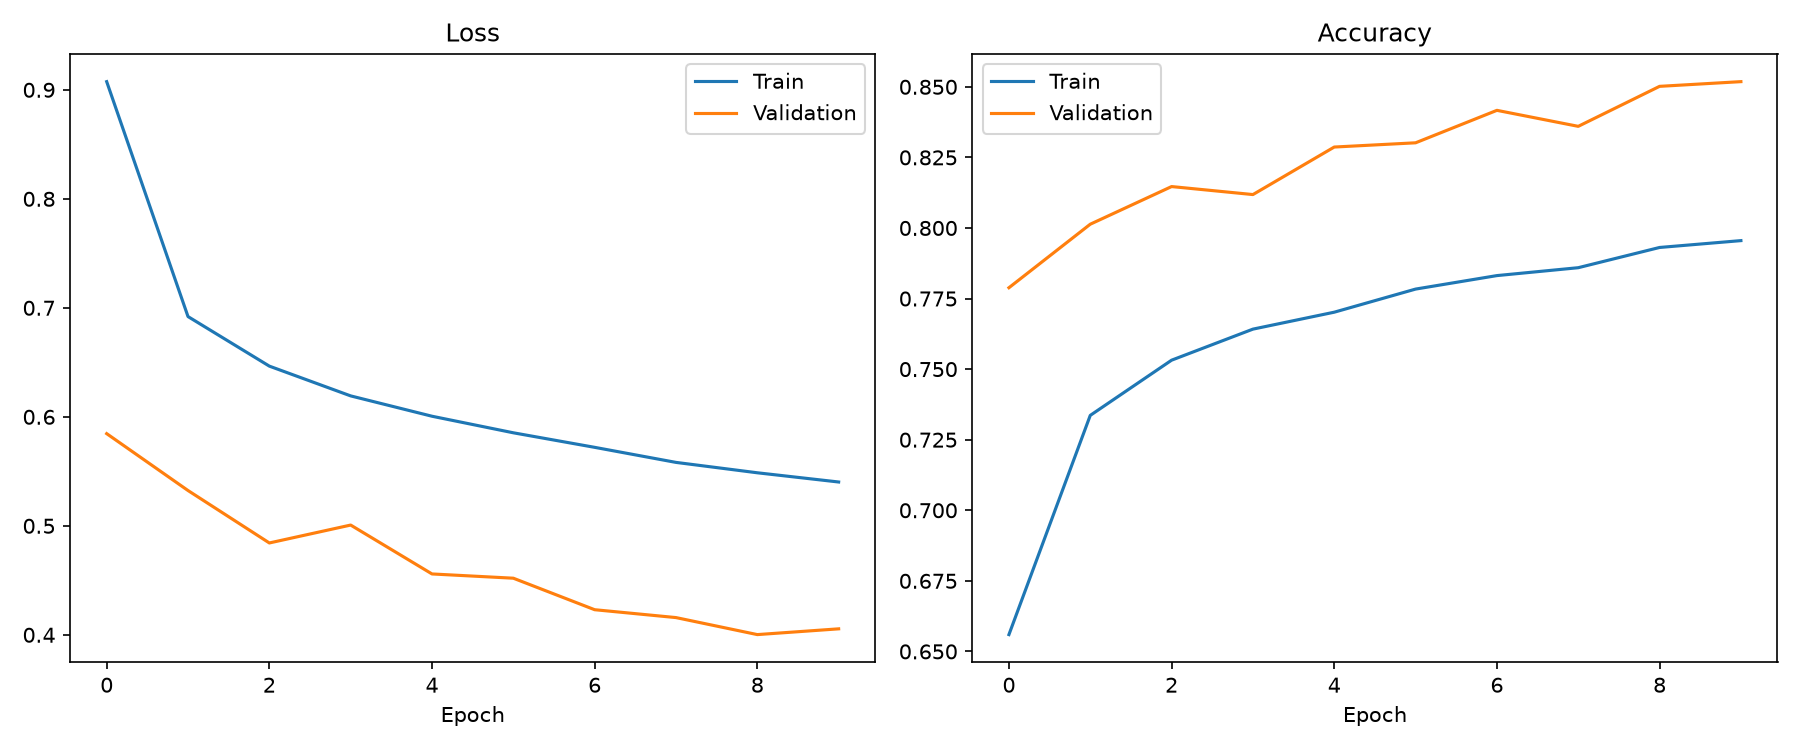
\includegraphics[width=0.9\textwidth]{../../Assignment1/outputs/learning_curves/mlp_learning_curves.png}
	\caption{MLP training and validation curves.}
	\label{fig:training-curves}
\end{figure}

The corresponding Linear learning curves are saved in 
\texttt{Assignment1/outputs/learning\_curves/linear\_learning\_curves.png}.
